\documentclass[a5paper, 10pt]{article}

\usepackage{cite, amsmath, amssymb, booktabs, lastpage, graphicx, float}
\usepackage[hidelinks]{hyperref}

\usepackage{geometry}
\geometry{margin=1.5cm,a5paper,twoside,inner=2cm}

\usepackage{setspace}
\usepackage{graphicx}
\makeatletter
\renewcommand{\maketitle}{
  \begin{center}
    \rule[.2em]{\textwidth}{0.353mm}
    \begin{minipage}[m]{0.35\textwidth}
      {\scriptsize
        \begin{center}
          \textsf{\textbf{\huge MATCH}\\
            \textit{Communications in Mathematical\\
              and in Computer Chemistry}}
        \end{center}}
    \end{minipage}\hfill
    \begin{minipage}[m]{0.65\textwidth}
      \begin{flushright}
        \baselineskip=10pt
        {\scriptsize\sffamily{\itshape MATCH Commun. Math. Comput. Chem.}
          \textbf{\vol{}}
          (\pubyear)
          \thepage--\pageref{LastPage}}\\
        {\scriptsize\sffamily {\bfseries ISSN:} 0340--6253}\\
        {\scriptsize\sffamily \textbf{doi:} \doi{10.46793/match.\vol-\num.\id}}
      \end{flushright}
    \end{minipage}
    \rule[1em]{\textwidth}{.353mm}
    \baselineskip=0.30in
    {\Large\bfseries \@title} \par
    \vspace{5mm}
    \baselineskip=0.2in
    {\large\bfseries \@author}\par
    \vspace{1mm}
    {\it \@address} \par
    {\small\tt \@email} \par
    \vspace{3mm}
    {\small (Received \@date)} \par
  \end{center}
  \vspace{3mm}
}
\newcommand{\address}[1]{\def\@address{#1}}
\newcommand{\email}[1]{\def\@email{#1}}
\newcommand{\doi}[1]{\href{https://doi.org/#1}{#1}}

\newcommand{\vol}{00}
\newcommand{\num}{00}
\newcommand{\pubyear}{0000}
\newcommand{\id}{xxxxx}
\setcounter{page}{1}
\thispagestyle{empty}
\makeatother

\newcommand{\acknowledgment}[1]{\vspace{5mm}\singlespacing
  {\noindent\textbf{\textit{Acknowledgment\/:}} #1}
}

\usepackage{fancyhdr}
\fancyhead{}
\fancyfoot{}
\renewcommand{\headrulewidth}{.3pt}
\voffset = 18pt
\headsep = 3pt
\renewcommand*{\thefootnote}{\fnsymbol{footnote}}
\usepackage[margin=1cm,font=footnotesize,format=hang,labelsep=period,labelfont=bf]{caption}
\fancyhead[RO]{\footnotesize \thepage}
\fancyhead[LE]{\footnotesize \thepage}
\pagestyle{fancy}

\usepackage{amsfonts}
\usepackage{subcaption}
\usepackage{multirow}
\usepackage{xcolor}
\usepackage{textcomp}
\usepackage{manyfoot}
\usepackage{algorithm}
\usepackage{algorithmicx}
\usepackage{algpseudocode}
\usepackage{listings}
\usepackage{tikz}
\usetikzlibrary{shapes.geometric, shapes.misc, arrows.meta, positioning}


\usepackage{array}

\title{Symmetry-Constrained Enumeration and Oriented Construction of Ordered MOF Candidates}

\author{Hui Li$^{a}$, Jing Tian$^{a,}$\footnote{Corresponding author.}, Dahuan Liu$^{a}$, Minman Tong$^{a}$, Qingyuan Yang$^{a}$}

\address{$^a$Beijing University of Chemical Technology, Beijing 100029, China}

\email{2024210575@buct.edu.cn}

\date{\today}


\begin{document}

\maketitle
\begin{abstract}
\setlength{\emergencystretch}{2em}

Metal-organic frameworks (MOFs) offer tunable structures for gas storage, catalysis, and separation, motivating systematic exploration of their building-unit arrangements. Assigning node types to the sites of a fixed MOF net produces different ordered arrangements. For such a net, we seek to identify assignments inequivalent under selected symmetries and construct periodic models with compatible building-unit connections and orientations.

We formulate degree-compatible node assignments as quotient-graph colorings, with a single fixed linker template on every edge. Selected orientation-preserving net symmetries define candidate equivalence. We organize fixed-point searches through the subgroup lattice and use depth-first search with canonical prefix comparisons to identify orbit representatives. Completed search regions are reused across tasks to avoid repeated exploration. Kabsch-based node alignment and linker placement construct oriented periodic models from selected representatives. In the geometric construction audit, models recovered the target topology, passed the short-contact check, and were exported as reloadable crystallographic information files (CIFs). We also used models constructed by this method for CO$_2$/N$_2$ adsorption screening and single-point density functional theory (DFT) energy comparisons within composition groups.
\end{abstract}
\onehalfspacing




\section{Introduction}
\label{sec:intro}
Metal-organic frameworks (MOFs) combine tunable porosity with diverse chemical functionality and are widely studied for gas storage, catalysis, and separation~\cite{furukawa2013chemistry}.
MOFs are assembled from modular building blocks, allowing even a finite library to yield millions of hypothetical frameworks~\cite{wilmer2012large}. High-throughput computational screening (HTCS) is therefore an important strategy for exploring this design space~\cite{colon2014high}.
Because screening evaluates generated structures, candidate generation must balance exploration with evaluation efficiency: it should propose varied building-unit arrangements, limit redundant candidates, and produce structural models suitable for downstream evaluation.%

Topology-based assembly methods such as ToBaCCo place building units on selected nets~\cite{colon2017topologically}. Reverse-topological methods match unit geometry to topological constraints~\cite{wu2024precisionmof}. Genetic algorithms have also been used to search MOF candidates by evolving encoded choices of topology and building units~\cite{pham2025genetic}. Deep generative models have expanded candidate proposal: MOFGPT uses language modeling~\cite{badrinarayanan2025mofgpt}, whereas MOFFlow uses flow matching~\cite{Kim2024MOFFlowFM}. MOFFLOW-2 couples building-unit generation in Simplified Molecular Input Line Entry System (SMILES) format with flow-matching assembly into three-dimensional frameworks~\cite{kim2025flexiblemof}.%

For candidate spaces defined by site assignments, symmetry-constrained enumeration limits redundancy by identifying assignments equivalent under a chosen symmetry group.
This approach is established for substitutional disorder in inorganic crystals~\cite{hart2012generating}. Hart--Forcade enumeration provides a framework for occupations on multicomponent parent crystals~\cite{hart2008algorithm}, and CASM implements occupation enumeration for first-principles studies of such crystals~\cite{PUCHALA2023111897}.%

On a fixed MOF net, node types can form distinct spatial arrangements at the same composition. The spatial arrangement of distinct building units is an important aspect of multicomponent MOF design~\cite{xu2020anisotropic}. A useful candidate set must distinguish patterns that are inequivalent under the chosen symmetry group. Each selected pattern must also map to a periodic model with compatible connection geometry and orientation for its secondary building units and linkers. Table~\ref{tab:related_capabilities} contrasts these approaches with our focus on identifying symmetry-distinct node assignments and constructing oriented periodic models on a fixed MOF net. %

\begin{table}[htbp]
\centering
\small
\singlespacing
\setlength{\tabcolsep}{5pt}
\renewcommand{\arraystretch}{1.08}
\captionsetup{margin=0pt,skip=6pt}
\caption{Design objects and principal operations of representative approaches to MOF candidate generation and crystal occupation enumeration.}
\label{tab:related_capabilities}
\begin{tabular}{@{}
    >{\raggedright\arraybackslash}p{\dimexpr0.18\linewidth-4\tabcolsep/3\relax}
    >{\raggedright\arraybackslash}p{\dimexpr0.27\linewidth-4\tabcolsep/3\relax}
    >{\raggedright\arraybackslash}p{\dimexpr0.55\linewidth-4\tabcolsep/3\relax}@{}}
\toprule
\textbf{Approach} & \textbf{Design object} & \textbf{Principal operation} \\
\midrule
Topology-based assembly & Selected nets, node units, and linkers. & Place building units on selected nets or match their geometry to topological constraints to construct periodic models. \\
\addlinespace[4pt]
Genetic algorithm search & Encoded choices of topology and building units. & Evolve candidate combinations, then construct and evaluate the resulting structures. \\
\addlinespace[4pt]
Deep generative models & Learned chemical and structural representations. & Propose candidates through language modeling or flow matching; MOFFLOW-2 couples building-unit generation with framework assembly. \\
\addlinespace[4pt]
Hart--Forcade / CASM & Species occupations on parent-crystal sites. & Enumerate configurations under parent-crystal symmetry. \\
\addlinespace[4pt]
This work & Node-type assignments on a fixed embedded MOF net. & Enumerate orbit representatives and construct oriented periodic models from selected assignments. \\
\bottomrule
\end{tabular}

\end{table}

We study node-type arrangements within a chosen repeat cell of a fixed embedded MOF net. A single linker template is held fixed on every edge throughout node-assignment enumeration.

The work makes two contributions:%
\begin{enumerate}
    \item In exhaustive runs, we organize deterministic fixed-point searches through the subgroup lattice and use canonical comparisons under the chosen symmetry group. This yields one representative per orbit and a candidate count specific to that group.
    \item Kabsch-based node alignment and linker placement construct oriented periodic models from selected representatives, with each model linked to its source assignment.
\end{enumerate}

\clearpage
\section{Candidate Enumeration and Model Construction}



\subsection{Coloring Space and Candidate Equivalence}


\label{sec:theory}
We fix the embedded net, a chosen repeat cell, and a single linker template used on every graph edge. The enumerated variable is the node-type label at each vertex; we call a labeling of all vertices a node assignment. The linker template is held fixed and is used only when constructing periodic models. We represent these node assignments in the chosen repeat cell as graph colorings. Figure~\ref{fig:pipeline} summarizes the full pipeline from this assignment space to a periodic model.

\begin{figure}[H]
    \centering
    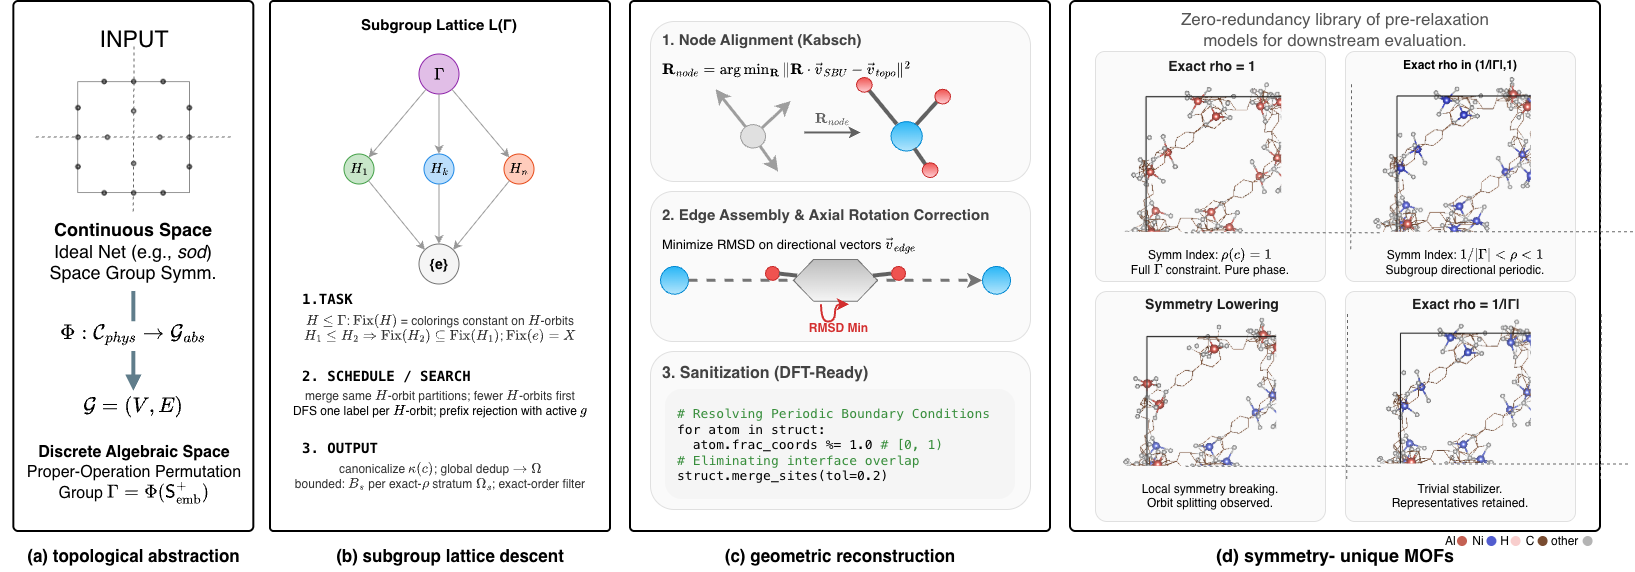
\includegraphics[width=\textwidth]{pipline.png}
    \caption{\textbf{Overview of the symmetry-constrained pipeline.} (a) Degree-compatible node labels define the assignment space; (b) subgroup fixed-point tasks return canonical representatives, with optional per-stratum quotas; (c) selected representatives are assembled by node alignment, linker placement, and sanitization; (d) representative pre-relaxation models labeled by exact $\rho$. A single linker template is fixed on all edges and not enumerated; symbols are defined in Sections 2.1--2.3.}
    \label{fig:pipeline}
\end{figure}

Let $\mathsf{T}\cong\mathbb{Z}^{3}$ be the translation subgroup generated by the lattice vectors of the chosen repeat cell. Factoring $\mathsf{T}$ out of the periodic net $\widetilde{Q}$ gives the finite quotient graph
\begin{equation}
Q=\widetilde{Q}/\mathsf{T}=(V,E).
\label{eq:quotient}
\end{equation}

The choice of $\mathsf{T}$ sets the translational periodicity of the assignments. If the repeat cell is a supercell, parent-net translations outside $\mathsf{T}$ connect positions represented by distinct vertices of $Q$. Independent labels on these vertices allow colorings that retain the repeat-cell periodicity while breaking shorter parent-net translations.

A vertex of $Q$ represents an orbit of positions under $\mathsf{T}$; all positions in that orbit receive the same label. For vertices of degree $d$, let $\mathcal{C}_d$ be the admissible node labels and $n_d$ the number of such vertices. We choose a label independently at each vertex, subject to its degree-specific pool. The set $X$ of all such node assignments is
\begin{equation}
X=\{c:V\to\cup_d\mathcal{C}_d\mid c(v)\in\mathcal{C}_{\deg(v)}\ \forall v\in V\},
\qquad |X|=\prod_d|\mathcal{C}_d|^{n_d}.
\label{eq:coloring_space}
\end{equation}

We compare assignments in $X$ under a finite group $\Gamma\leq\mathrm{Sym}(V)$ of degree-preserving vertex permutations.
Here $\Gamma$ is the permutation image of the orientation-preserving crystallographic operations of the embedded net (Section~\ref{sec:reconstruction_method}). Assignments related only by a reflection are therefore kept distinct unless an orientation-preserving operation maps one to the other.

The action of each $g\in\Gamma$ moves labels with their vertices, giving
\begin{equation}
(g\cdot c)(v)=c(g^{-1}v),\qquad
\mathcal{O}_{\Gamma}(c)=\{g\cdot c:g\in\Gamma\}.
\label{eq:group_action}
\end{equation}
Because $\Gamma$ preserves degrees, this action maps $X$ to itself. Assignments in the same $\Gamma$-orbit are treated as one candidate, while different orbits remain distinct even at the same composition. Thus $N_\Gamma=|X/\Gamma|$, and changing $\Gamma$ can change the candidate count. For $\Gamma_1\leq\Gamma_2$ acting on the same $X$, each $\Gamma_2$-orbit is a union of $\Gamma_1$-orbits, giving $N_{\Gamma_2}\leq N_{\Gamma_1}$.


Fix a vertex order $v_1,\ldots,v_{|V|}$ and a total order on labels, and compare colorings lexicographically in these orders. Canonical comparisons use the lexicographic order of label strings. Depth-first search (DFS) visits the admissible labels in their supplied pool order, which determines the traversal sequence within each task. The least coloring in each orbit is its canonical representative:
\begin{equation}
\kappa(c)=\min_{g\in\Gamma}(g\cdot c),\qquad
\Omega=\{\kappa(c):c\in X\},\qquad |\Omega|=|X/\Gamma|.
\label{eq:canonical_rep}
\end{equation}

For a coloring $c\in X$, the operations in $\Gamma$ that preserve $c$ form its stabilizer subgroup. The orbit--stabilizer relation gives its relative size $\rho(c)$:
\begin{equation}
\mathrm{Stab}_{\Gamma}(c)=\{g\in\Gamma:g\cdot c=c\},\qquad
\rho(c)=\frac{|\mathrm{Stab}_{\Gamma}(c)|}{|\Gamma|}
=\frac{1}{|\mathcal{O}_{\Gamma}(c)|}.
\label{eq:stabilizer_rho}
\end{equation}
Here, $\rho$ is the fraction of group elements preserving $c$. Stabilizers within an orbit are conjugate, making their order and $\rho$ well defined for each candidate.


\subsection{Enumeration by Subgroup-Lattice Descent}


\label{sec:enumeration}
Each coloring is fixed by its stabilizer subgroup, so subgroup operations can be imposed as constraints during enumeration. For a chosen $H\leq\Gamma$, the constraint is $c(hv)=c(v)$ for every $h\in H$ and $v\in V$. Let $\mathcal{P}_H=\{Hv:v\in V\}$ denote the distinct $H$-orbits on $V$. A coloring fixed by $H$ is constant on each $P\in\mathcal{P}_H$. Since $H\leq\Gamma$ preserves degrees, all vertices in each $P$ have a common degree, denoted $\deg(P)$. Assigning one admissible label to each $H$-orbit gives the fixed-point domain
\begin{equation}
\begin{aligned}
\mathrm{Fix}(H)&=\{c\in X:H\leq\mathrm{Stab}_{\Gamma}(c)\}\\
&\cong\prod_{P\in\mathcal{P}_H}\mathcal{C}_{\deg(P)},\\
|\mathrm{Fix}(H)|&=\prod_d|\mathcal{C}_d|^{m_{H,d}},
\end{aligned}
\label{eq:fixed_layer}
\end{equation}
where $m_{H,d}$ counts the degree-$d$ vertex orbits in $\mathcal{P}_H$. The cardinality of this domain counts assignments before $\Gamma$-equivalence reduction.

If $H_1\leq H_2$, every coloring fixed by $H_2$ is also fixed by $H_1$, giving $\mathrm{Fix}(H_2)\subseteq\mathrm{Fix}(H_1)$. Each $H_2$-orbit is a union of $H_1$-orbits, so the weaker constraints for $H_1$ allow labels to vary between those smaller orbits. At the identity subgroup $\{e\}$, every vertex is a singleton orbit and $\mathrm{Fix}(\{e\})=X$.

The subgroups ordered by inclusion form the subgroup lattice of $\Gamma$. Algorithm~\ref{alg:enum} constructs fixed-point tasks from their vertex-orbit partitions, including the full-group and identity tasks. Identical partitions among proper nontrivial subgroup tasks are merged. Tasks are searched in increasing order of the number of vertex orbits, beginning with the full-group partition; ties retain the construction order.

Different subgroup tasks can have overlapping fixed-point domains. After a task has been searched to completion, its vertex-orbit partition is recorded as a set of equal-label constraints. A later branch is rejected when every completion satisfies the constraints of an already completed task. This coverage test can discard an entire branch before a complete assignment is formed.

Within each task, depth-first search assigns labels one $H$-orbit at a time. At an intermediate state, a partial coloring $c_p$ records admissible labels on an assigned set $D_p\subseteq V$ and the marker $\bot$ elsewhere. A completion within the current $H$-task is a coloring $c\in\mathrm{Fix}(H)$ satisfying $c(v)=c_p(v)$ for every $v\in D_p$.

The canonical minimum in Eq.~\ref{eq:canonical_rep} allows early rejection when assigned labels force a smaller $\Gamma$-image for every completion of a branch.
For each $g\in\Gamma$, compare $c_p(v_i)$ and $c_p(g^{-1}v_i)$ in the fixed vertex order. For this $g$, the common assigned prefix is the longest initial segment with $v_i,g^{-1}v_i\in D_p$ at every position. Comparison stops before the first unassigned entry; $\bot$ does not participate in label comparisons. Reject the branch if some $g\in\Gamma$ and $1\leq j\leq |V|$ satisfy%
\begin{equation}
\begin{aligned}
v_i,\ g^{-1}v_i&\in D_p &&(1\leq i\leq j),\\
c_p(g^{-1}v_i)&=c_p(v_i) &&(1\leq i<j),\\
c_p(g^{-1}v_j)&<c_p(v_j).
\end{aligned}
\label{eq:prefix_rejection}
\end{equation}
Every completion agrees with $c_p$ on $D_p$ and therefore inherits the comparison at the first differing position $j$ in the common assigned prefix. If $c_p(g^{-1}v_j)<c_p(v_j)$, then $g\cdot c<_{\mathrm{lex}}c$ for every completion: the branch contains no canonical representative and is rejected. If $c_p(g^{-1}v_j)>c_p(v_j)$, then $g\cdot c>_{\mathrm{lex}}c$ for every completion: $g$ cannot produce a smaller image, so it is removed from the active comparison set while the branch remains searchable.

For each operation in the active comparison set, the search stores the end of the vertex prefix already confirmed to be equal. Descendant states resume comparison from that position, and backtracking restores the comparison state. At a complete surviving leaf, the coloring is already the canonical representative. The active set $\mathcal{A}$ then contains exactly the nonidentity operations that fix this coloring, giving
\begin{equation}
 s(c)=|\mathrm{Stab}_{\Gamma}(c)|=1+|\mathcal{A}|,
 \qquad |\Gamma\cdot c|=\frac{|\Gamma|}{s(c)}.
\label{eq:active_stabilizer}
\end{equation}
In exhaustive enumeration, each complete canonical representative is retained once, together with its stabilizer order and orbit size.

\medskip
\noindent\textbf{Completeness.}
The identity task has domain $\mathrm{Fix}(\{e\})=X$, so every canonical representative lies in its search space. Canonical prefix rejection removes only branches whose completions have a smaller $\Gamma$-image. Coverage rejection removes a branch only after its canonical search has been completed in an earlier task or subtree. Each canonical representative is therefore either retained earlier or remains reachable in the identity task. The global membership check records it once. With quotas, output caps, and task timeouts disabled and all tasks searched to completion, the algorithm returns every member of $\Omega$ exactly once.

A representative with full stabilizer order $s$ belongs to the candidate stratum $\Omega_s$:
\begin{equation}
\begin{aligned}
\Omega_s&=\{c^\star\in\Omega:|\mathrm{Stab}_{\Gamma}(c^\star)|=s\},\\
\Omega&=\bigsqcup_s\Omega_s,\qquad
\rho(c^\star)=s/|\Gamma|\quad(c^\star\in\Omega_s).
\end{aligned}
\label{eq:rho_strata}
\end{equation}

For large assignment spaces, the user may bound output by specifying an exact-$\rho$ quota $B_s$ for each stabilizer stratum $\Omega_s$. The search retains the same fixed-point constraints and canonical prefix comparisons. When quotas are enabled, tasks are ordered by decreasing subgroup order, with identical partitions merged within each order and the remaining partitions searched lexicographically. An order-$s$ task retains a canonical representative only when its full stabilizer order equals $s$. Only newly retained representatives count towards $B_s$.

When quotas are enabled, coverage records are shared only among tasks targeting the same stabilizer order. A completed task certifies that all representatives in its fixed-point domain belonging to that stratum have been processed. Changing the target order starts a new set of coverage records, while previously retained representatives remain available for global deduplication.

\medskip
\noindent\textbf{Bounded output.}
Task deadlines and a total output cap may further limit the search. An interrupted task contributes coverage records only for its completed subtrees. Such a record can be reused when every completion of a later branch satisfies the source task's fixed-point constraints, lies within its admissible label domains, and matches the completed prefix. In quota-controlled searches, reuse remains restricted to the same target stabilizer order.

If no task times out and $M_{\mathrm{total}}\geq\sum_sB_s$, stratum $s$ returns the first $\min\{B_s,|\Omega_s|\}$ representatives in the fixed task and vertex-orbit orders, with labels visited in their supplied pool order. Reaching $B_s$ fills the quota; completing all tasks for that stratum before filling the quota establishes exhaustion. The coverage and sequence guarantees are proved in Supplementary Section~\ref{app:quota_proof}.

\begin{algorithm}[H]
\caption{Subgroup-Lattice Descent}
\label{alg:enum}
\scriptsize
\setlength{\baselineskip}{7.1pt}
\begin{algorithmic}[1]
\Require $\Gamma$; degree-typed label pools $\{\mathcal C_d\}$; optional quotas $B_s$, task deadline and total output cap
\Ensure Distinct retained representatives with stabilizer orders and orbit sizes
\State initialize records $R$, membership set $K$, coverage records $C$, and stratum counts $N_s\gets0$
\State build raw tasks $Q_0=\{(\mathcal P_H,|H|)\}$ for the full group, identity and proper subgroups
\State write $\mathcal P=(P_0,\ldots,P_{m-1})$, ordering blocks by their smallest vertex index
\State form $Q$ from $Q_0$, merging proper-subgroup partitions; prioritize fewer vertex orbits, retaining construction order for ties
\If{quotas are enabled}
  \State rebuild $Q$ from $Q_0$, merging within each subgroup order; search orders decreasingly and partitions lexicographically
\EndIf
\For{each task $(\mathcal P,s)$ in $Q$, where $s$ is the source subgroup order}
  \State \textbf{if} total output cap reached \textbf{then break}
  \State \textbf{if} quotas enabled and $N_s\ge B_s$ \textbf{then continue}
  \State \textbf{if} quotas enabled and target order changes \textbf{then} clear $C$
  \State initialize $c_p$, $\mathcal A\gets\Gamma\setminus\{e\}$, cursors $\boldsymbol\ell\gets\mathbf0$, and task deadline
  \State compile eligible coverage checks for $\mathcal P$; initialize completed-choice progress
  \State $state\gets$ \Call{CanonicalDFS}{$0,c_p,\mathcal A,\boldsymbol\ell,\mathcal P,s$}
  \State register completed task or subtree coverage in $C$ according to $state$ and the saved frontier
\EndFor
\State stable-sort $R$ by decreasing stabilizer order; \Return $R$
\Statex
\Function{CanonicalDFS}{$k,c_p,\mathcal A,\boldsymbol\ell,\mathcal P,s$}
  \State \textbf{if} an applicable time or output limit is reached \textbf{then} save frontier; \Return OPEN
  \State \textbf{if} eligible coverage contains every completion \textbf{then} \Return CLOSED
  \If{$k=|\mathcal P|$}
    \State $t\gets1+|\mathcal A|$
    \State \textbf{if} quotas enabled and $t\ne s$ \textbf{then} \Return CLOSED
    \If{$c_p\notin K$}
      \State insert $c_p$ into $K$; append $(c_p,t,|\Gamma|/t)$ to $R$; $N_t\gets N_t+1$
    \EndIf
    \State \Return CLOSED
  \EndIf
  \State initialize completed-choice progress at this level
  \For{each admissible label for $P_k$ in the supplied order}
    \State \textbf{if} a limit is reached \textbf{then} save frontier; \Return OPEN
    \State assign the label to $P_k$; $\mathcal A'\gets\emptyset$; $\boldsymbol\ell'\gets\boldsymbol\ell$; $rejected\gets false$
    \For{each $g\in\mathcal A$}
      \State compare from $\ell_g+1$, stopping at an unassigned pair or the first unequal pair
      \If{the first difference gives a smaller image}
        \State $rejected\gets true$; \textbf{break}
      \ElsIf{no difference was reached}
        \State retain $g$ in $\mathcal A'$; advance $\ell'_g$ to the end of the confirmed equal prefix
      \EndIf
    \EndFor
    \State $child\gets CLOSED$
    \If{not $rejected$}
      \State $child\gets$ \Call{CanonicalDFS}{$k+1,c_p,\mathcal A',\boldsymbol\ell',\mathcal P,s$}
    \EndIf
    \State restore assignment and comparison state
    \State \textbf{if} $child=OPEN$ \textbf{then} \Return OPEN
    \State mark the label choice completed
  \EndFor
  \State \Return CLOSED
\EndFunction
\end{algorithmic}
\end{algorithm}

\subsection{Crystallographic Symmetry and Geometric Construction}



\label{sec:reconstruction_method}
The crystallographic symmetries of the embedded net induce vertex permutations in the chosen repeat cell. We use their orientation-preserving permutation image as $\Gamma$.

Let $\mathsf{S}_{\mathrm{emb}}^{+}$ denote the orientation-preserving crystallographic operations of the embedded net that preserve $\mathsf{T}$ and the degree-typed label pools. Each operation $q$ induces the vertex permutation $\Phi(q)(v)=[q\widetilde v]_{\mathsf T}$, where $\widetilde v$ represents the periodic position associated with $v$. Their permutation image is
\begin{equation}
\Gamma=\Phi(\mathsf{S}_{\mathrm{emb}}^{+})\leq\mathrm{Sym}(V).
\label{eq:rotation_group}
\end{equation}
Parent translations outside $\mathsf{T}$ can induce nontrivial permutations within the repeat cell, while the embedding excludes graph automorphisms that are not crystallographic symmetries of the periodic net.
We retain only proper operations because template placement uses proper rotations ($\det R=1$) to align oriented connection vectors; a reflection would reverse template handedness.

The implementation derives candidate permutations from the crystallographic operations of the embedded vertex set. The selection and matching steps are summarized in Algorithm~\ref{alg:gamma_construction}. Use of the resulting permutation set as $\Gamma$ requires group closure, degree preservation, and quotient-graph adjacency preservation. Supplementary Section~\ref{app:benchmark_symmetry} reports the group orders, generators, and operation-selection counts for the three benchmark nets. These properties were independently checked for all three resulting permutation sets.

\begin{algorithm}[htbp]
\caption{Numerical generation of candidate embedded-net permutations}
\label{alg:gamma_construction}
\scriptsize
\begin{algorithmic}[1]
\Require Lattice and fractional coordinates $\{x_i\}_{i=1}^{|V|}$ of the embedded vertices
\Ensure Candidate set $P$ of unique proper-operation permutations
\State Build the periodic structure using the implementation's placeholder species: Zn if a node symbol contains Z or M, and C otherwise
\State $\mathcal{O}^*\gets\emptyset$; $n^*\gets0$
\For{$\delta\in(0.01,0.1,0.3)\,\text{\AA}$, in ascending order}
    \State $\mathcal{O}_{\delta}\gets$ \texttt{SpacegroupAnalyzer} operations at $\texttt{symprec}=\delta$ (default angle tolerance $5^\circ$; continue if analysis fails)
    \If{$|\mathcal{O}_{\delta}|>n^*$}
        \State $(\mathcal{O}^*,n^*)\gets(\mathcal{O}_{\delta},|\mathcal{O}_{\delta}|)$
    \EndIf
    \If{$|\mathcal{O}_{\delta}|>16$} \State \textbf{break} \EndIf
\EndFor
\If{no operation set was obtained} \State \Return $\{e\}$ \EndIf
\State $P\gets\emptyset$
\For{each $q\in\mathcal{O}^*$ with $\det R_q\geq0$}
    \State Map each $q x_i$ to the first index $j$ with periodic distance $d_{ij}<0.8\,\text{\AA}$
    \If{every vertex is mapped and the map is bijective} \State add its permutation to $P$ \EndIf
\EndFor
\State $P\gets\operatorname{sort}(P\cup\{e\})$ after removing duplicates
\State \Return $P$
\end{algorithmic}
\end{algorithm}

For a selected canonical representative $c^\star$, the vertex labels specify node templates at graph vertices. The same linker template is used on every graph edge when constructing the periodic model; it is not enumerated in $X$. The periodic embedding supplies placement centers and connection vectors. Node and linker templates retain their specified conformations. Connection-site labels beginning with \texttt{X} mark the atoms used for attachment; they retain their template chemical species during placement. When needed, the repeat cell is uniformly expanded to accommodate the required connections, with a 5\% buffer on the expansion factor.

For each node, let $p_i$ denote a template connection-site vector relative to the centroid of its connection sites. We take $a_i$ to point from the embedded vertex to the position of the adjacent vertex. The candidate correspondences are the bijections between the template connection sites and the incident network vectors. For each bijection, Kabsch alignment~\cite{kabsch1976solution,lawrence2019kabschumeyama} determines the least-squares proper rotation%
\begin{equation}
R^\star=\underset{R^{\mathsf T}R=I,\;\det R=1}{\operatorname{arg\,min}}
\sum_i\lVert R p_i-a_i\rVert^2.
\label{eq:kabsch_alignment}
\end{equation}

The root mean square deviation (RMSD) of the aligned vectors ranks the bijections. The rotation yielding the lowest RMSD is applied to every template atom, with ties resolved by the fixed site order; the connection-site centroid is placed at the embedded vertex. The constraint $\det R=1$ preserves template handedness during placement.%

Each linker is aligned along the axis joining its connection anchors, with periodic images chosen to match the neighboring node endpoints. Interfragment bridge bonds are constructed using periodic endpoint distances and connection-count constraints, with distance-based repair of missing node--linker connections. Discrete rotations about the linker endpoint axis are then evaluated to reduce nonbonded clashes while retaining the template conformation.

After these rotations, the geometric audit measures the actual separations of topology-linked node--linker \texttt{X}--\texttt{X} pairs before endpoint fusion. Node-side and linker-side \texttt{X} endpoints with a Cartesian separation strictly below $0.8\,\text{\AA}$ are then merged one-to-one. After fusion, the remaining topology-linked pairs define the bridge connections. Their CIF bond-table entries use a nominal length of $1.485\,\text{\AA}$ without displacing the atomic coordinates. The numerical criteria are listed in Supplementary Section~\ref{app:reconstruction_protocol}. Appendix~\ref{app:x_fusion} reports the fixed-geometry scan of the fusion cutoff.

\begingroup\setlength{\emergencystretch}{1em}
Residual dummy sites with chemical species \texttt{X} are then removed. Framework sites within $0.2\,\text{\AA}$ are merged to eliminate coincident coordinates. The resulting periodic pre-relaxation model is exported as a CIF linked to $c^\star$ for structural audit and downstream screening.
\par\endgroup

\section{Results}

The \texttt{ffc} and \texttt{fjh} nets were used for exhaustive enumeration benchmarks, and \texttt{vba} was used to examine bounded output across symmetry strata. The timing benchmarks varied the sizes of the degree-compatible node-label pools; their exact membership is recorded in Supplementary Section~\ref{app:enum_benchmark}. Models for construction audits and property screening used the separately specified building-unit pools in Supplementary Table~\ref{tab:building_units}, with \texttt{1B\_4H\_Ch} fixed as the linker on every edge.

\subsection{Exact and External Enumeration Checks}

For each exhaustive case, distinct canonical representatives defined disjoint $\Gamma$-orbits whose sizes summed to $|X|$, confirming complete coverage. The matched CASM workflow used the same assignment space, group action, and output fields. After normalization to a common canonical convention, the complete representative records agreed.

Enumeration wall times were lower for this method in 5 of the eight \texttt{ffc} and \texttt{fjh} cases in Table~\ref{tab:casm}. In the largest \texttt{fjh} case, 16,777,216 assignments yielded 1,078,816 orbits in 2.74 s, compared with 20.88 s for CASM. CASM was faster in the three smallest assignment spaces. These measurements support generating complete candidate libraries over the tested spaces, with relative performance dependent on the case.

CASM's native full factor group $F$ additionally includes orientation-reversing operations. Its orbit counts are reported separately in Supplementary Table~\ref{tab:orbit_group_counts}, showing the effect of the equivalence group.

\begin{table}[H]
\centering\scriptsize
\setlength{\tabcolsep}{1.2mm}
\caption{\textbf{Matched-group enumeration on benchmark quotient graphs.} Both workflows use the same $\Gamma$ and return complete assignments, stabilizer orders, and orbit sizes. Times are enumeration wall-time medians of three single-threaded runs. Input pools and timing boundaries are specified in Supplementary Section~\ref{app:enum_benchmark}.}
\label{tab:casm}
\begin{tabular}{llrrrr}
\toprule
Net & $|\mathcal C_3|/|\mathcal C_4|$ & $|X|$ & Orbits & This work (s) & CASM (s) \\
\midrule
\texttt{ffc} & 2/2 & 128 & 42 & 0.004731 & 0.0002792 \\
\texttt{ffc} & 3/3 & 2,187 & 513 & 0.00515 & 0.003053 \\
\texttt{ffc} & 5/5 & 78,125 & 14,250 & 0.01491 & 0.0942 \\
\texttt{ffc} & 5/15 & 2,109,375 & 381,375 & 0.5123 & 2.636 \\
\texttt{fjh} & 1/2 & 4,096 & 394 & 0.04508 & 0.005913 \\
\texttt{fjh} & 2/1 & 65,536 & 4,756 & 0.04954 & 0.09325 \\
\texttt{fjh} & 1/3 & 531,441 & 36,369 & 0.119 & 0.6977 \\
\texttt{fjh} & 1/4 & 16,777,216 & 1,078,816 & 2.74 & 20.88 \\
\bottomrule
\end{tabular}
\end{table}


The 32 vertices of \texttt{vba} admit $2^{32}$ or $3^{32}$ assignments for the two node-label pools. Table~\ref{tab:vba_bounded} compares per-stratum quotas with DFS prefixes containing the same total number of representatives. The ordered label pools and run settings are specified in Supplementary Section~\ref{app:enum_benchmark}. The quota runs retained representatives from every exact-$\rho$ stratum, including the trivial-stabilizer stratum $\rho=1/16$; the matched DFS prefixes omitted that stratum. The quota guarantee classifies entries below $B_s$ as exhausted and entries at $B_s$ as quota-filled. Neither quota run timed out or reached the global cap. The representatives retained across strata provide a bounded candidate set for subsequent periodic model construction.
\begin{table}[H]
\centering
\scriptsize
\setlength{\tabcolsep}{2.5mm}
\renewcommand{\arraystretch}{1.2}
\caption{\textbf{Bounded \texttt{vba} output across exact-$\rho$ strata.} For each node-label pool, the DFS prefix and per-stratum quota contain the same total number of representatives. The two quota runs used $B_s=20{,}000$, $M_{\mathrm{total}}=100{,}000$, and a 60\,s limit per task. Parentheses give the number of distinct node-label count vectors in each stratum; layer times for the per-stratum quota policy are medians of three runs for the layer intervals defined in Supplementary Section~\ref{app:enum_benchmark}.}
\label{tab:vba_bounded}
\begin{tabular}{llccc}
\toprule
\textbf{Pool} & $\boldsymbol{\rho}$ & \textbf{DFS prefix} & \textbf{Per-$\rho$ quota} & \textbf{Layer time (s)} \\
\midrule
\multicolumn{5}{l}{$|\mathcal{C}_4|=2$; matched total = 41,984} \\
$|\mathcal C_4|=2$ & $1$ & 4\;(3) & 4\;(3) & 0.0002 \\
$|\mathcal C_4|=2$ & $0.5$ & 90\;(3) & 90\;(3) & 0.0012 \\
$|\mathcal C_4|=2$ & $0.25$ & 1,890\;(7) & 1,890\;(7) & 0.0080 \\
$|\mathcal C_4|=2$ & $0.125$ & 40,000\;(15) & 20,000\;(15) & 0.0183 \\
$|\mathcal C_4|=2$ & $0.0625$ & 0\;(0) & 20,000\;(15) & 0.0157 \\
\addlinespace
\multicolumn{5}{l}{$|\mathcal{C}_4|=3$; matched total = 60,549} \\
$|\mathcal C_4|=3$ & $1$ & 9\;(6) & 9\;(6) & 0.0002 \\
$|\mathcal C_4|=3$ & $0.5$ & 540\;(12) & 540\;(12) & 0.0016 \\
$|\mathcal C_4|=3$ & $0.25$ & 55,440\;(42) & 20,000\;(42) & 0.0193 \\
$|\mathcal C_4|=3$ & $0.125$ & 4,560\;(43) & 20,000\;(54) & 0.0149 \\
$|\mathcal C_4|=3$ & $0.0625$ & 0\;(0) & 20,000\;(54) & 0.0395 \\
\bottomrule
\end{tabular}%
\end{table}

\subsection{Geometric Construction Audit}
\label{sec:reconstruction}

Periodic atomic models were constructed from the canonical ordering representatives to test whether their assigned building units could realize the intended network connectivity. For the construction audit, the \texttt{ffc} pool comprised \texttt{3c\_B\_Ch} and \texttt{3c\_triazine\_Ch} at three-connected vertices, and \texttt{4c\_B\_Ch} and \texttt{4c\_Cd\_1\_Ch} at four-connected vertices. The \texttt{fjh} pool used \texttt{3c\_B\_Ch} at three-connected vertices and the same two four-connected templates. All 42 \texttt{ffc} representatives and a fixed-seed sample of 30 out of 394 \texttt{fjh} representatives were assembled successfully. Each model produced a sanitized, reloadable CIF, recovered the target topology, and passed the short-contact check. These results establish successful transfer from discrete assignments to periodic structures for the 72 tested cases. Figure~\ref{fig:reconstruction_gallery} illustrates constructed models from all three benchmark nets; the quantitative audit covers \texttt{ffc} and \texttt{fjh}.

The node--linker bridge lengths quantify how closely rigid building-unit placement matches the target connection geometry. Across 3,888 topology-linked \texttt{X}--\texttt{X} pairs, the RMSD from the nominal $1.485$\,\AA{} bridge length was 0.388\,\AA{}. The fusion tolerance is 0.8\,\AA{}. Separately, the closure audit measures the actual \texttt{X}--\texttt{X} separation against the nominal $1.485$\,\AA{} bridge length; 95.7\% of separations lie within a 0.8\,\AA{} deviation window. Together with topology recovery and the short-contact check, these measurements support using the constructed models as periodic starting structures for downstream calculations. Structural relaxation remains a subsequent step. The contact criterion and sample selection are detailed in Supplementary Section~\ref{app:reconstruction_audit}.


\begin{figure}[htbp]
    \centering
    \begin{subfigure}[t]{0.32\linewidth}
        \centering
        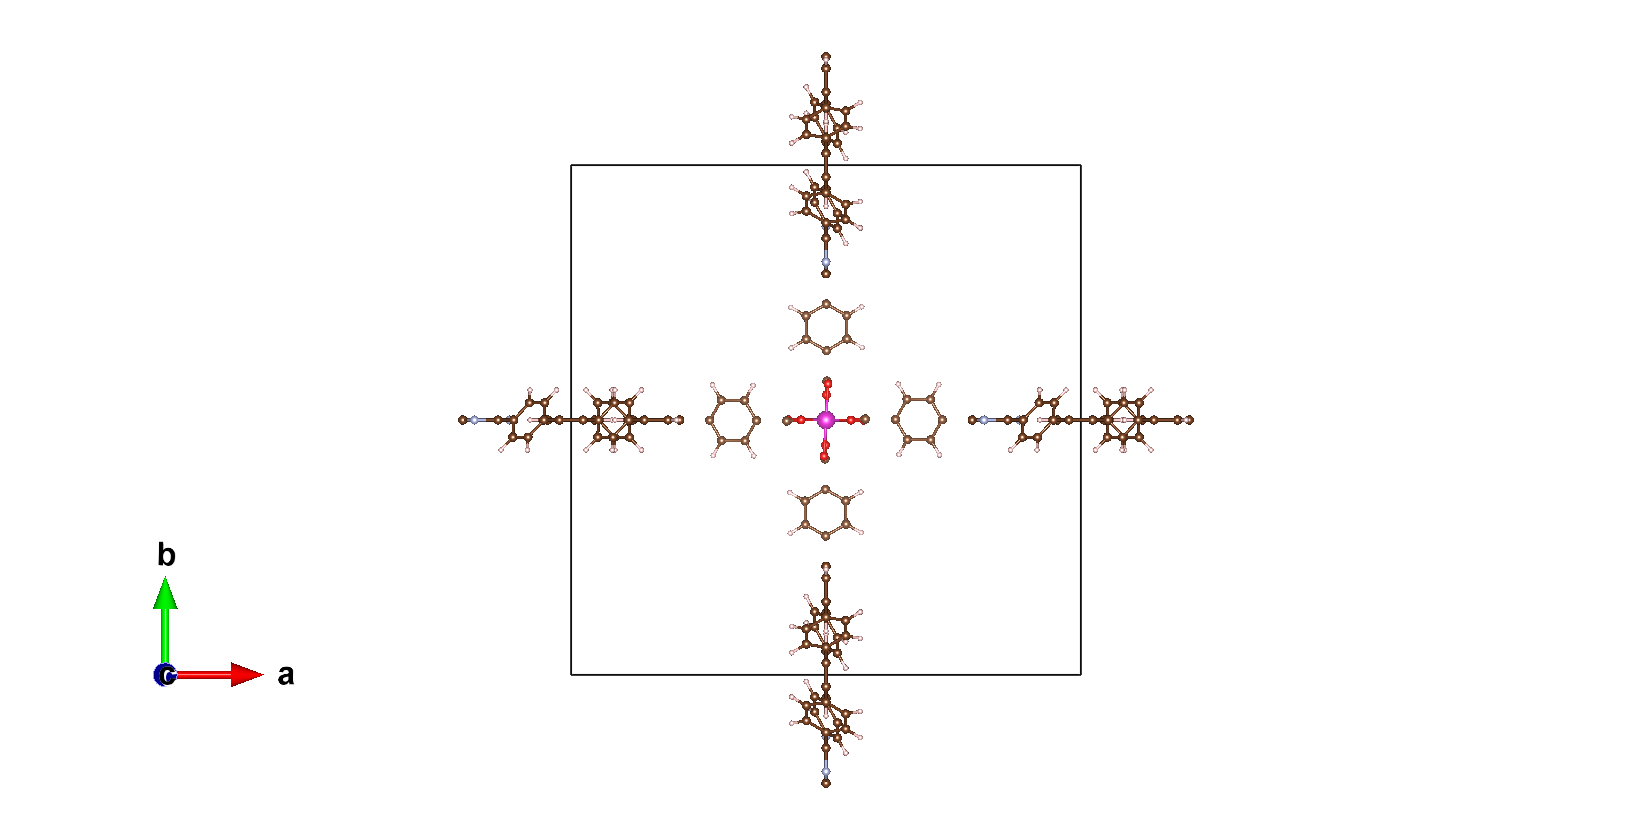
\includegraphics[width=\linewidth,trim={400bp 35bp 350bp 35bp},clip]{ffc_comp_b_21.png}
        \caption*{\textbf{(a)}\quad\texttt{ffc}}
    \end{subfigure}
    \hfill
    \begin{subfigure}[t]{0.32\linewidth}
        \centering
        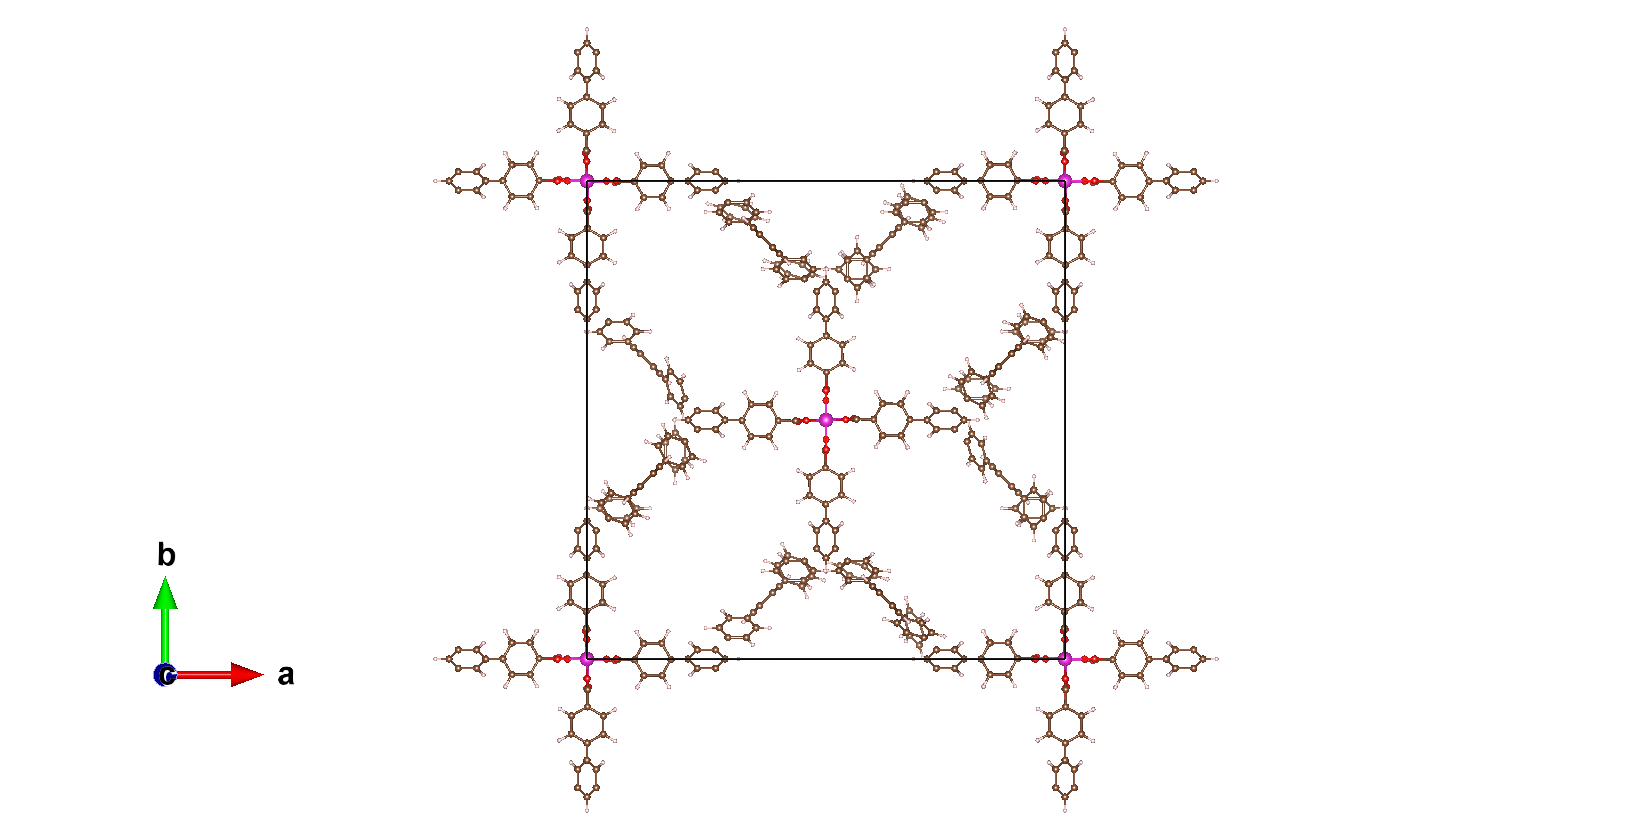
\includegraphics[width=\linewidth,trim={400bp 20bp 350bp 20bp},clip]{fjh_comp_b_1.png}
        \caption*{\textbf{(b)}\quad\texttt{fjh}}
    \end{subfigure}
    \hfill
    \begin{subfigure}[t]{0.32\linewidth}
        \centering
        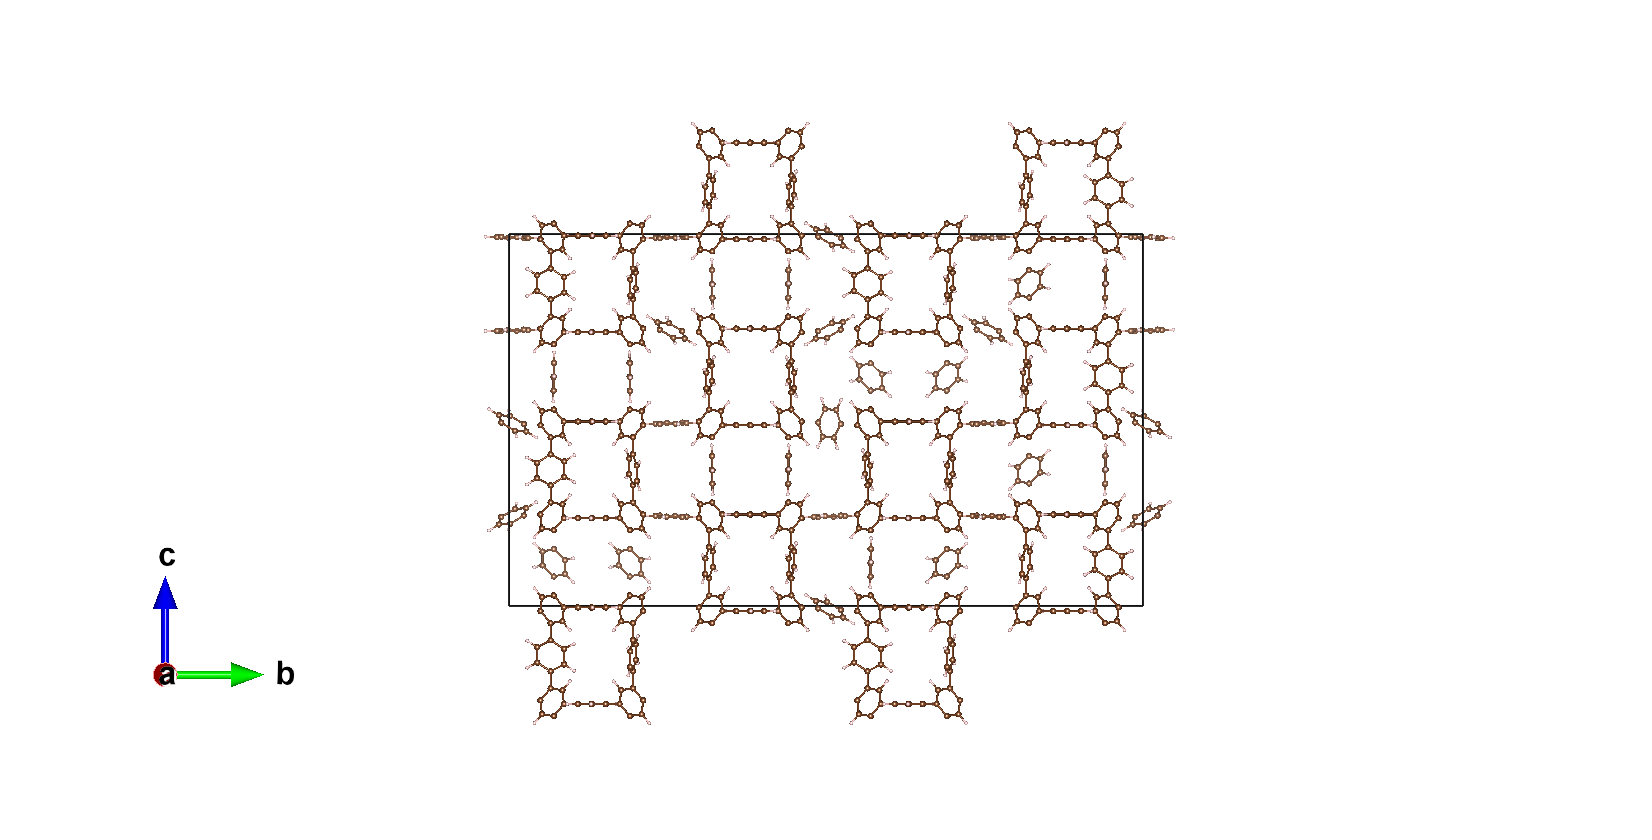
\includegraphics[width=\linewidth,trim={400bp 90bp 450bp 90bp},clip]{vba_rho1.png}
        \caption*{\textbf{(c)}\quad\texttt{vba}}
    \end{subfigure}
    \caption{Representative pre-relaxation crystal models constructed from symmetry-distinct assignments in \texttt{ffc}, \texttt{fjh}, and \texttt{vba}.}
    \label{fig:reconstruction_gallery}
\end{figure}

\subsection{Downstream Screening of Constructed Models}
\label{sec:screening}
\subsubsection{\texorpdfstring{CO$_2$/N$_2$ Adsorption Screening}{CO2/N2 Adsorption Screening}}

The \texttt{ffc} models were grouped by node composition and exact $\rho$, retaining groups with at least three successfully screened ordering representatives. This matching holds composition and stabilizer fraction fixed while comparing spatial arrangements. The group compositions are listed in Supplementary Table~\ref{tab:adsorption_group_compositions}. Zeo++ supplied the pore-limiting diameter (PLD) and largest-cavity diameter (LCD) of the corresponding constructed models~\cite{willems2012algorithms}.

Grand canonical Monte Carlo (GCMC) simulations in RASPA2 estimated equilibrium CO$_2$/N$_2$ adsorption by sampling molecular exchange with a gas reservoir~\cite{dubbeldam2016raspa,altintas2018database}. For species $i$, let $q_i(p)$ be its adsorbed loading at pressure $p$ and $y_i$ its gas-phase mole fraction. With adsorption and desorption pressures $p_{\mathrm{ads}}$ and $p_{\mathrm{des}}$, the screening metrics are
\begin{equation}
\label{eq:co2_metrics}
\begin{aligned}
S &= \frac{q_{\mathrm{CO_2}}(p_{\mathrm{ads}})/q_{\mathrm{N_2}}(p_{\mathrm{ads}})}{y_{\mathrm{CO_2}}/y_{\mathrm{N_2}}},\\
WC &= q_{\mathrm{CO_2}}(p_{\mathrm{ads}})-q_{\mathrm{CO_2}}(p_{\mathrm{des}}),\\
R &= \frac{WC}{q_{\mathrm{CO_2}}(p_{\mathrm{ads}})},\\
APS &= S\times WC.
\end{aligned}
\end{equation}
The selectivity $S$ measures preferential CO$_2$ adsorption, and $WC$ measures the loading released over the pressure swing. The working-capacity fraction $R$ expresses that release relative to the adsorption loading; the adsorbent performance score $APS$ combines selectivity and capacity~\cite{altintas2018database,avci2018high}. Numerical conditions and the averaging protocol are given in Supplementary Section~\ref{app:adsorption_screening}.

\begin{table}[htbp]
\centering
\scriptsize
\caption{\textbf{Pore geometry and CO$_2$/N$_2$ screening within matched \texttt{ffc} ordering groups.} The 30 models form nine groups of fixed node composition and exact $\rho$; $n$ counts symmetry-distinct orderings per group. Entries give within-group minimum--maximum ranges. For each model, $WC$, $S$, and $R$ are means over five independent GCMC runs; $APS$ is mean $S$ times mean $WC$. Across the nine groups, within-group spans range from 0.019 to 0.100 mmol\,g$^{-1}$ for $APS$, 0.03 to 1.02~\AA{} for PLD, and 0.18 to 0.92~\AA{} for LCD, calculated before rounding.}
\label{tab:ffc_co2n2_ordering}
\setlength{\tabcolsep}{0.6mm}
\renewcommand{\arraystretch}{1.12}
\begin{tabular}{@{}lcccccccc@{}}
\toprule
\textbf{Group} & \textbf{$\rho$} & \textbf{$n$} & \textbf{PLD} & \textbf{LCD} & \textbf{WC} & \textbf{S} & \textbf{R} & \textbf{APS} \\
 & & & (\AA) & (\AA) & (mmol\,g$^{-1}$) & (1) & (1) & (mmol\,g$^{-1}$) \\
\midrule
G1 & 0.125 & 3 & 26.44--26.97 & 27.68--28.00 & 0.083--0.091 & 1.915--2.104 & 0.896--0.904 & 0.158--0.192 \\
G2 & 0.25 & 4 & 26.41--27.07 & 27.39--28.27 & 0.084--0.092 & 1.939--2.110 & 0.897--0.901 & 0.163--0.194 \\
G3 & 0.125 & 3 & 26.36--26.51 & 27.85--28.20 & 0.085--0.090 & 1.898--1.996 & 0.900--0.903 & 0.160--0.180 \\
G4 & 0.25 & 3 & 26.38--26.41 & 27.39--28.31 & 0.092--0.100 & 2.019--2.151 & 0.894--0.905 & 0.188--0.214 \\
G5 & 0.25 & 3 & 27.01--27.06 & 27.93--28.20 & 0.084--0.089 & 1.909--2.022 & 0.898--0.901 & 0.161--0.180 \\
G6 & 0.25 & 3 & 27.01--27.06 & 27.93--28.20 & 0.092--0.097 & 1.881--1.992 & 0.899--0.904 & 0.174--0.192 \\
G7 & 0.50 & 4 & 26.15--26.83 & 27.36--27.79 & 0.082--0.093 & 1.923--2.112 & 0.896--0.904 & 0.157--0.196 \\
G8 & 0.50 & 4 & 25.80--26.81 & 27.31--27.78 & 0.085--0.098 & 1.954--2.128 & 0.897--0.906 & 0.166--0.209 \\
G9 & 0.50 & 3 & 26.50--26.74 & 27.45--27.63 & 0.097--0.118 & 2.206--2.662 & 0.892--0.906 & 0.213--0.313 \\
\bottomrule
\end{tabular}
\end{table}

Within the matched groups, distinct ordering representatives can differ in pore dimensions and mean adsorption metrics (Table~\ref{tab:ffc_co2n2_ordering}). Fixing composition and exact $\rho$ therefore still leaves geometrically distinct candidates for screening. The highest-$APS$ ordering was unchanged across all five runs in only two groups, indicating that most within-group rankings were sensitive to simulation runs. The observed geometric differences and run-sensitive rankings support evaluating the retained orderings individually under the screening protocol.


\subsubsection{Single-point DFT Energy Screening}

A separate set of constructed \texttt{ffc} and \texttt{fjh} models was evaluated with single-point PBE+D3 calculations to compare ordering energies at fixed composition. The atomic coordinates were held fixed, so the comparison evaluates the geometries supplied by construction. Within each sampled composition, the relative energy $\Delta E$ is the per-atom energy difference from the lowest-energy model.

The composition-controlled panels in Fig.~\ref{fig:symmetry_screening} show energy differences among the retained orderings, with composition minima occurring in multiple $\rho$ strata. Retaining representatives across symmetry strata provides alternatives for energy comparisons within each sampled composition. These calculations demonstrate the connection from canonical assignments through periodic construction to electronic-structure screening; the rankings concern the sampled starting geometries before relaxation. Computational settings are given in Supplementary Section~\ref{app:dft_screening}.

\begin{figure}[htbp]
    \centering
    \begin{subfigure}[t]{0.495\linewidth}
        \centering
        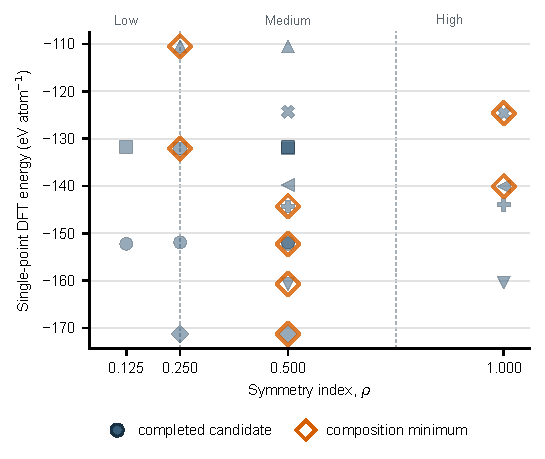
\includegraphics[width=\linewidth]{ffc_pooled_symmetry_energy_a.pdf}
        \caption{Pooled energies, \texttt{ffc}.}
    \end{subfigure}
    \hfill
    \begin{subfigure}[t]{0.495\linewidth}
        \centering
        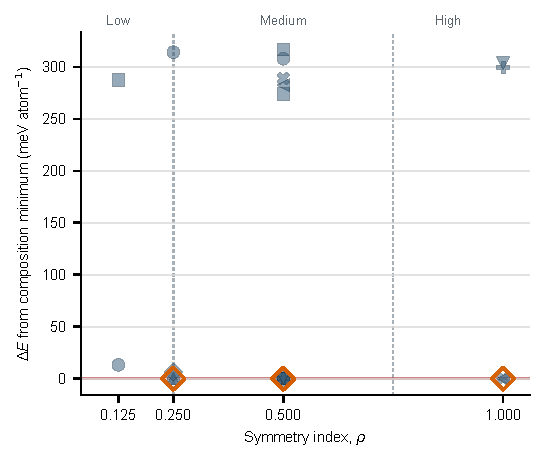
\includegraphics[width=\linewidth]{ffc_pooled_symmetry_energy_b.pdf}
        \caption{Composition-controlled $\Delta E$, \texttt{ffc}.}
    \end{subfigure}

    \vspace{0.35em}

    \begin{subfigure}[t]{0.495\linewidth}
        \centering
        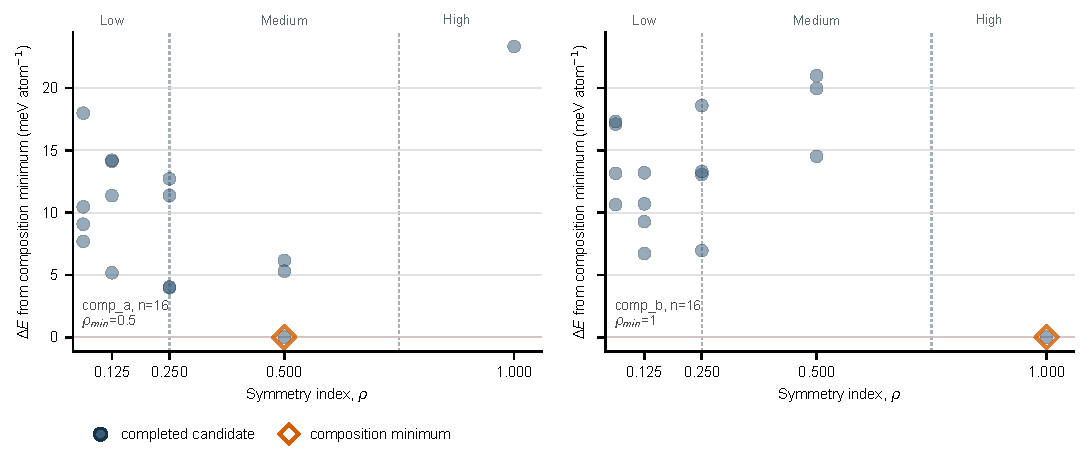
\includegraphics[width=\linewidth,trim={0 0 262 0},clip]{fjh_dual_delta_symmetry_energy.pdf}
        \caption{Composition-controlled $\Delta E$, \texttt{fjh comp\_a}.}
    \end{subfigure}
    \hfill
    \begin{subfigure}[t]{0.495\linewidth}
        \centering
        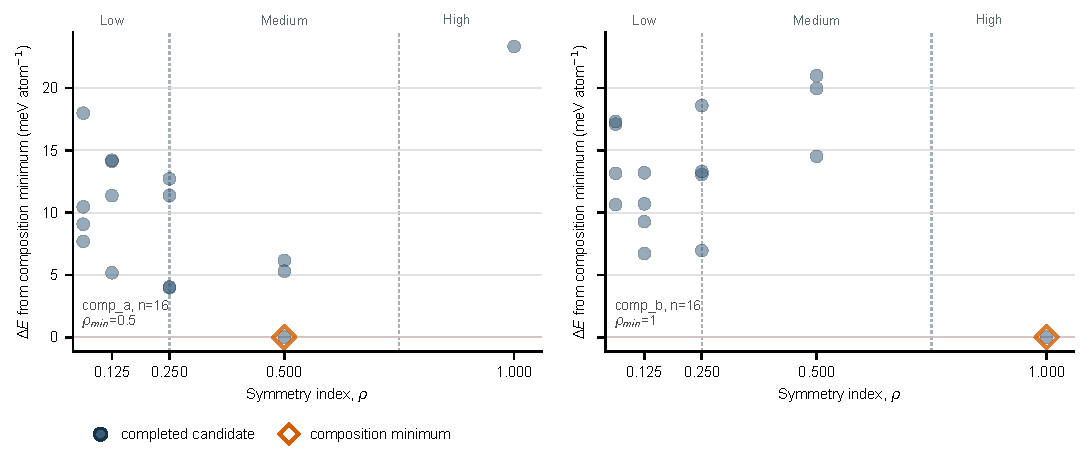
\includegraphics[width=\linewidth,trim={262 0 0 0},clip]{fjh_dual_delta_symmetry_energy.pdf}
        \caption{Composition-controlled $\Delta E$, \texttt{fjh comp\_b}.}
    \end{subfigure}
    \caption{\textbf{Single-point DFT screening of constructed \texttt{ffc} and \texttt{fjh} models.} PBE+D3 calculations converged for all 21 \texttt{ffc} models from eight composition groups and all 32 \texttt{fjh} models from two fixed compositions: \texttt{comp\_a} (16 \texttt{3c\_B\_Ch}, 4 \texttt{4c\_B\_Ch}, and 8 \texttt{4c\_Cd\_1\_Ch}) and \texttt{comp\_b} (16 \texttt{3c\_B\_Ch}, 8 \texttt{4c\_B\_Ch}, and 4 \texttt{4c\_Cd\_1\_Ch}). Panel (a) pools the \texttt{ffc} per-atom energies (eV\,atom$^{-1}$) across compositions; panels (b)--(d) show $\Delta E$ (meV\,atom$^{-1}$), the per-atom energy relative to the lowest value in each sampled composition. Filled-marker shapes distinguish compositions, and open orange diamonds mark their minima. Vertical guides indicate low ($\rho<0.25$), medium ($0.25\le\rho\le0.75$), and high ($\rho>0.75$) $\rho$ ranges.}
    \label{fig:symmetry_screening}
\end{figure}

\section{Conclusion}
\label{sec:discussion}
In exhaustive runs, the method returns one representative per $\Gamma$-orbit. The matched-group benchmarks support its use for generating symmetry-distinct candidate libraries over the tested assignment spaces. Selected representatives are then used to construct pre-relaxation periodic models for subsequent screening.

The 72-model audit established successful construction from discrete assignments. Separate matched screening sets demonstrated the use of constructed models for downstream evaluation. Within the matched adsorption groups, distinct orderings can differ in pore descriptors and protocol-specific mean screening metrics, although the highest-APS ordering was unchanged across all five runs in only two of the nine groups. Separate single-point DFT calculations compared the energies of constructed orderings within fixed-composition groups. The evaluated models are pre-relaxation starting structures; whether distinct models remain structurally distinct and stable after relaxation requires further evaluation.

\section*{Data Availability}
\label{sec:data}
The code and data supporting the reported enumeration, model construction, adsorption, and single-point DFT results are available in the \href{https://github.com/Buct454/mof-enumeration-reconstruction.git}{GitHub repository}. The package includes representative and audited CIF models, source tables for the matched-group CASM benchmarks and DFT energies, CO$_2$/N$_2$ screening data, bounded-\texttt{vba} records, and the X-site fusion audit. Versioned benchmark records, input pools, and source snapshots document the reported enumeration results. The README and file manifest map these data to the manuscript figures and tables. All deposited CIFs are pre-relaxation starting models.

\acknowledgment{This work was supported by the National Key R\&D Program of China (No. 2021YFB3802200).}

\section*{Author Contributions}
H.L. conceived the study. H.L. and J.T. developed the algorithm, implemented the workflow, and performed the computational experiments. D.L., M.T., and Q.Y. contributed to method discussion, result interpretation, and manuscript refinement. All authors discussed the results, reviewed the manuscript, and approved the final version.


\section*{Competing Interests}
The authors declare that they have no competing financial interests, personal relationships, or other conflicts of interest that could have influenced the work reported in this manuscript.



\singlespacing

\bibliographystyle{unsrt}
\bibliography{reference}


\clearpage
\appendix
\section{Supplementary Information}
\label{app:supplementary}
\setcounter{equation}{0}
\renewcommand{\theequation}{A\arabic{equation}}
\renewcommand{\theHequation}{A.\arabic{equation}}
\setcounter{table}{0}
\renewcommand{\thetable}{A\arabic{table}}
\renewcommand{\theHtable}{A.\arabic{table}}
\setcounter{figure}{0}
\renewcommand{\thefigure}{A\arabic{figure}}
\renewcommand{\theHfigure}{A.\arabic{figure}}
\subsection{Building-unit templates}
\label{app:building_units}

Table~\ref{tab:building_units} lists the ten node templates used for model construction and screening, together with the fixed linker template. The adsorption set contains all ten node types. Enumeration timing benchmarks additionally used larger degree-compatible label pools, whose membership is listed in Supplementary Section~\ref{app:enum_benchmark}.

\begin{table}[H]
\centering
\scriptsize
\setlength{\tabcolsep}{1.2mm}
\renewcommand{\arraystretch}{1.15}
\caption{Node and linker templates used for model construction and screening.}
\label{tab:building_units}
\begin{tabular}{@{}p{0.32\linewidth}p{0.16\linewidth}p{0.46\linewidth}@{}}
\toprule
\textbf{Template} & \textbf{Type} & \textbf{Role in this study} \\
\midrule
\texttt{3c\_B\_Ch} & 3-connected node & Enumeration, construction, and screening \\
\texttt{3c\_pyrrole\_Ch} & 3-connected node & CO$_2$/N$_2$ adsorption screening \\
\texttt{3c\_triazine\_Ch} & 3-connected node & Enumeration, construction, and screening \\
\texttt{4c\_B\_Ch} & 4-connected node & Enumeration, construction, and screening \\
\texttt{4c\_Cd\_1\_Ch} & 4-connected node & Construction and screening \\
\texttt{4c\_Cu\_1\_Ch} & 4-connected node & Construction, adsorption screening, and visual examples \\
\texttt{4c\_In\_1\_Ch} & 4-connected node & CO$_2$/N$_2$ adsorption screening \\
\texttt{4c\_Ni\_1\_Ch} & 4-connected node & CO$_2$/N$_2$ adsorption screening \\
\texttt{4c\_V\_1\_Ch} & 4-connected node & CO$_2$/N$_2$ adsorption screening \\
\texttt{4c\_tetrathiafulvalene\_Ch} & 4-connected node & CO$_2$/N$_2$ adsorption screening \\
\texttt{1B\_4H\_Ch} & Linker & Fixed edge template in all constructed models \\
\bottomrule
\end{tabular}
\end{table}

\subsection{Benchmark symmetry groups}
\label{app:benchmark_symmetry}

The benchmark symmetry operations were determined from the sorted vertex coordinates and lattice vectors in each graph input. To construct periodic structures for symmetry analysis, vertices with symbols containing Z or M were assigned Zn, and all other vertices were assigned C. For all three nets, the selected crystallographic operation sets used a positional tolerance of 0.01\,\AA{} and an angular tolerance of $5^\circ$. The reported space-group symbols describe these placeholder structures. An operation was included when its rotation determinant was positive and its periodic vertex map was bijective; operations with negative determinant were excluded to preserve orientation. No operation failed vertex matching or bijectivity in these benchmarks. The listed generators are affine operations on fractional coordinates; their induced permutations generate the reported $\Gamma$. Independent checks confirmed that each resulting permutation set is closed and preserves vertex degrees and quotient-graph adjacency.

\begin{table}[htbp]
\centering
\scriptsize
\setlength{\tabcolsep}{3pt}
\renewcommand{\arraystretch}{1.15}
\caption{Benchmark permutation-group orders and operation selection. Candidate operations are those in the selected placeholder-structure symmetry set.}
\label{tab:benchmark_symmetry}
\begin{tabular}{@{}lccp{0.34\linewidth}p{0.30\linewidth}@{}}
\toprule
Net & $|V|$ & $|\Gamma|$ & Selected placeholder space group & Included / excluded operations \\
\midrule
\texttt{ffc} & 7 & 8 & $P4/mmm$ ($16$ operations) & $8$ included ($\det R>0$); $8$ excluded ($\det R<0$); $0$ other rejections \\
\texttt{fjh} & 28 & 16 & $I4/mcm$ ($32$ operations) & $16$ included ($\det R>0$); $16$ excluded ($\det R<0$); $0$ other rejections \\
\texttt{vba} & 32 & 16 & $Fddd$ ($32$ operations) & $16$ included ($\det R>0$); $16$ excluded ($\det R<0$); $0$ other rejections \\
\bottomrule
\end{tabular}
\end{table}

\begin{table}[H]
\centering
\scriptsize
\setlength{\tabcolsep}{4pt}
\renewcommand{\arraystretch}{1.2}
\caption{Generating crystallographic operations for the benchmark permutation groups. Each listed operation acts on fractional coordinates modulo lattice translations.}
\label{tab:benchmark_generators}
\begin{tabular}{@{}lp{0.78\linewidth}@{}}
\toprule
Net & Generating operations $q_i:(x,y,z)\mapsto(x',y',z')$ \\
\midrule
\texttt{ffc} & \shortstack[l]{$q_1:(x,y,z)\mapsto(-x,y,-z)$\\$q_2:(x,y,z)\mapsto(x,-y,-z)$\\$q_3:(x,y,z)\mapsto(y,x,-z)$} \\
\texttt{fjh} & \shortstack[l]{$q_1:(x,y,z)\mapsto(-y,x,z)$\\$q_2:(x,y,z)\mapsto(x,-y,-z+\tfrac12)$\\$q_3:(x,y,z)\mapsto(-y+\tfrac12,-x+\tfrac12,-z)$} \\
\texttt{vba} & \shortstack[l]{$q_1:(x,y,z)\mapsto(-x+\tfrac34,-y+\tfrac34,z)$\\$q_2:(x,y,z)\mapsto(-x+\tfrac34,y,-z+\tfrac34)$\\$q_3:(x,y,z)\mapsto(-x+\tfrac34,y+\tfrac12,-z+\tfrac14)$\\$q_4:(x,y,z)\mapsto(-x+\tfrac14,y,-z+\tfrac14)$} \\
\bottomrule
\end{tabular}
\end{table}

\subsection{Enumeration implementation}
\label{app:enumeration_implementation}

\begingroup\setlength{\emergencystretch}{3em}
Python prepares the subgroup tasks and their coverage constraints. A C++ kernel performs depth-first assignment, canonical prefix comparisons, stabilizer extraction, and complete-representative membership checks. When quotas are enabled, the kernel additionally receives the target stabilizer order and remaining layer budget. Records are returned in batches and decoded and sorted in Python.
\par\endgroup

\begingroup\setlength{\emergencystretch}{3em}
\subsection{Matched-group enumeration benchmarks}
\label{app:enum_benchmark}

The enumeration benchmarks used the current ABI-4 implementation snapshot, Python 3.11.1, and CASM 2.3.1, with OMP, OpenBLAS, and MKL thread counts set to one. CPU affinity was not pinned. The recorded platform was macOS 26.6.2 on arm64; the archived native build script specifies C++17 with \texttt{-O3} optimization. The implementation tested here used the C++ DFS backend and the path-compressed representative index, with completed-prefix caching enabled. The CASM workflow called its occupation counter and canonical-configuration test with a subgroup whose site permutations matched $\Gamma$, and constructed the same output fields: the complete assignment, stabilizer order, and orbit size. Count-only timings under $\Gamma$ were measured separately.

Wall times are medians of three independent sequential runs. Dependency imports, graph and group construction, and verification were outside the timed interval; subgroup-task preparation, search, result storage, decoding, and sorting were included where performed. All exhaustive attempts finished within the external limits of 180\,s and 1536\,MiB per process, with internal output budgets and task timeouts disabled. Representative counts agreed with independent Burnside calculations, orbit sizes summed to $|X|$, and complete records agreed after normalization to the same canonical convention.

For each degree, the timing pools were prefixes of the available template filenames in lexicographic order. Both workflows used the same pools, with cardinalities given in Table~\ref{tab:casm} and Supplementary Table~\ref{tab:matched_extra}. The ordered master lists were:

\noindent $\mathcal{C}_{3}$ ordered master list:
\begin{center}\small
\begin{tabular}{rl}
1 & \texttt{3c\_B\_Ch} \\
2 & \texttt{3c\_Cu\_imadazoline\_Ch} \\
3 & \texttt{3c\_pyrrole\_Ch} \\
4 & \texttt{3c\_triazine\_Ch} \\
5 & \texttt{3c\_uranyl} \\
\end{tabular}
\end{center}

\noindent $\mathcal{C}_{4}$ ordered master list:
\begin{center}\small
\begin{tabular}{rl}
1 & \texttt{4c\_1anC\_Ch} \\
2 & \texttt{4c\_4B\_fused\_Ch} \\
3 & \texttt{4c\_B\_Ch} \\
4 & \texttt{4c\_Cd\_1\_Ch} \\
5 & \texttt{4c\_Cu\_1\_Ch} \\
6 & \texttt{4c\_In\_1\_Ch} \\
7 & \texttt{4c\_Ni\_1\_Ch} \\
8 & \texttt{4c\_V\_1\_Ch} \\
9 & \texttt{4c\_Zn\_tet} \\
10 & \texttt{4c\_bicyclooctane\_Ch} \\
11 & \texttt{4c\_ethene\_Ch} \\
12 & \texttt{4c\_porphyrin\_Ch} \\
13 & \texttt{4c\_pyrene\_Ch} \\
14 & \texttt{4c\_pyrene\_NU\_Ch} \\
15 & \texttt{4c\_tetrathiafulvalene\_Ch} \\
\end{tabular}
\end{center}

The bounded \texttt{vba} runs used the first two or three labels of the same ordered $\mathcal C_4$ master list. Canonical comparisons used label-string lexicographic order, and DFS visited labels in the listed order. Both policies used the ABI-4 C++ backend with the representative index and completed-prefix cache enabled. Quota runs used $B_s=20{,}000$, a total cap of 100,000, and a 60\,s task limit; DFS prefixes stopped at the corresponding quota run's total output. No task timed out. Layer times are medians of three independent runs and include the work performed within each layer; initial subgroup setup is outside those layer intervals.

These benchmarks enumerated assignments without constructing atomic models. The construction-audit pools are specified separately in Section~\ref{sec:reconstruction}.

\begin{table}[H]
\centering\scriptsize
\setlength{\tabcolsep}{1.2mm}
\caption{Matched-group enumeration with complete representative records. Times are enumeration wall times; CASM uses the same $\Gamma$.}
\label{tab:matched_extra}
\begin{tabular}{llrrrr}
\toprule
Net & $|\mathcal C_3|/|\mathcal C_4|$ & $|X|$ & Orbits & This work (s) & CASM (s) \\
\midrule
\texttt{ffc} & 2/2 & 128 & 42 & 0.004731 & 0.0002792 \\
\texttt{ffc} & 3/3 & 2,187 & 513 & 0.00515 & 0.003053 \\
\texttt{ffc} & 5/5 & 78,125 & 14,250 & 0.01491 & 0.0942 \\
\texttt{ffc} & 5/15 & 2,109,375 & 381,375 & 0.5123 & 2.636 \\
\texttt{fjh} & 1/2 & 4,096 & 394 & 0.04508 & 0.005913 \\
\texttt{fjh} & 2/1 & 65,536 & 4,756 & 0.04954 & 0.09325 \\
\texttt{fjh} & 1/3 & 531,441 & 36,369 & 0.119 & 0.6977 \\
\texttt{fjh} & 1/4 & 16,777,216 & 1,078,816 & 2.74 & 20.88 \\
\texttt{lil} & 4/3 & 5,308,416 & 1,328,832 & 1.978 & 6.858 \\
\bottomrule
\end{tabular}
\end{table}

An additional \texttt{lil} case used $|\mathcal C_3|=4$, $|\mathcal C_4|=3$, and $|\Gamma|=4$. This case tested enumeration on a further net; no atomic models were constructed for it.

CASM's native full factor group $F$ also includes orientation-reversing operations. Under $F$, the \texttt{ffc} orbit counts matched those under $\Gamma$ for the tested pools, whereas the \texttt{fjh} counts were smaller. For \texttt{fjh} 1/4, the counts were 577,456 under $F$ and 1,078,816 under $\Gamma$. These counts describe the effect of the selected equivalence group; the matched-group timings in this section use $\Gamma$ on both sides.

\begin{table}[H]
\centering\scriptsize
\setlength{\tabcolsep}{1.2mm}
\caption{Assignment-orbit counts under the orientation-preserving group $\Gamma$ and the native full factor group $F$.}
\label{tab:orbit_group_counts}
\begin{tabular}{llrr}
\toprule
Net & $|\mathcal C_3|/|\mathcal C_4|$ & Orbits ($\Gamma$) & Orbits ($F$) \\
\midrule
\texttt{ffc} & 2/2 & 42 & 42 \\
\texttt{ffc} & 3/3 & 513 & 513 \\
\texttt{ffc} & 5/5 & 14,250 & 14,250 \\
\texttt{ffc} & 5/15 & 381,375 & 381,375 \\
\texttt{fjh} & 1/2 & 394 & 265 \\
\texttt{fjh} & 2/1 & 4,756 & 2,476 \\
\texttt{fjh} & 1/3 & 36,369 & 20,655 \\
\texttt{fjh} & 1/4 & 1,078,816 & 577,456 \\
\texttt{lil} & 4/3 & 1,328,832 & 667,872 \\
\bottomrule
\end{tabular}
\end{table}

Peak process memory was 921.2\,MiB for this work and 734.1\,MiB for CASM in the largest \texttt{fjh} case. The completed-prefix cache had no hits in the timed runs. Process memory includes interpreter and dependency allocations through enumeration completion; it is distinct from the logical size of the representative index.

\begin{table}[H]
\centering\scriptsize
\setlength{\tabcolsep}{1.2mm}
\caption{Observed wall-time ranges over three runs and peak process memory medians. Time ranges are in seconds and memory is in MiB.}
\begin{tabular}{llrrrr}
\toprule
Net & Pool & Time range (ours) & Time range (CASM) & RSS (ours) & RSS (CASM) \\
\midrule
\texttt{ffc} & 2/2 & 0.004529--0.004801 & 0.0002756--0.0003917 & 143.9 & 142.0 \\
\texttt{ffc} & 3/3 & 0.005073--0.00527 & 0.002942--0.003115 & 143.8 & 143.3 \\
\texttt{ffc} & 5/5 & 0.01471--0.01499 & 0.09231--0.1014 & 149.6 & 145.2 \\
\texttt{ffc} & 5/15 & 0.5049--0.5139 & 2.612--2.662 & 377.2 & 276.2 \\
\texttt{fjh} & 1/2 & 0.04423--0.04549 & 0.005912--0.00593 & 145.0 & 142.9 \\
\texttt{fjh} & 2/1 & 0.04908--0.04958 & 0.09037--0.1113 & 146.5 & 142.8 \\
\texttt{fjh} & 1/3 & 0.1138--0.1208 & 0.6882--0.7228 & 172.6 & 162.2 \\
\texttt{fjh} & 1/4 & 2.74--2.746 & 20.54--21.11 & 921.2 & 734.1 \\
\texttt{lil} & 4/3 & 1.867--2.057 & 6.825--6.969 & 855.3 & 700.6 \\
\bottomrule
\end{tabular}
\end{table}

\begin{table}[H]
\centering\scriptsize
\setlength{\tabcolsep}{1.2mm}
\caption{Native-core time of this work and a separate CASM count-only comparison under $\Gamma$ (seconds, medians of three runs). Native-core time is a subset of enumeration wall time.}
\begin{tabular}{llrr}
\toprule
Net & Pool & Native core (ours) & CASM count only \\
\midrule
\texttt{ffc} & 2/2 & 5.25e-05 & 0.0001502 \\
\texttt{ffc} & 3/3 & 0.0001472 & 0.001801 \\
\texttt{ffc} & 5/5 & 0.001824 & 0.06066 \\
\texttt{ffc} & 5/15 & 0.04905 & 1.623 \\
\texttt{fjh} & 1/2 & 0.000874 & 0.004513 \\
\texttt{fjh} & 2/1 & 0.001904 & 0.07653 \\
\texttt{fjh} & 1/3 & 0.03399 & 0.5555 \\
\texttt{fjh} & 1/4 & 0.838 & 17.23 \\
\texttt{lil} & 4/3 & 0.1648 & 3.722 \\
\bottomrule
\end{tabular}
\end{table}

\endgroup

\subsection{Bounded output and exact-$\rho$ quotas}
\label{app:quota_proof}

We prove the coverage and prefix guarantee stated in Section~\ref{sec:enumeration}. Quota setup starts from cyclic subgroups and repeatedly takes proper pairwise joins. The cyclic subgroups generated by elements of any $S<\Gamma$ join to $S$, and all intermediate joins remain in $S$; $\Gamma$ is added separately. Within each order, tasks with identical vertex-orbit partitions are merged and the remaining partitions are searched lexicographically.

For $c^\star\in\Omega_s$, let $S=\mathrm{Stab}_{\Gamma}(c^\star)$. The task for $S$ contains $c^\star$, and its canonical minimality protects the corresponding branch from prefix rejection. Coverage rejection can remove this branch only after $c^\star$ has been processed under the same target order. Otherwise the search reaches the leaf, which satisfies the exact-order acceptance rule.

A coverage record for target order $s$ certifies that every member of $\Omega_s$ in its source task or completed subtree has been processed. If all completions of a later branch satisfy the source fixed-point and label-domain constraints and lie in that recorded region, the branch contains no new eligible representative. Same-order partition merging preserves the source domain. These coverage checks therefore preserve the new representatives and their order of acceptance.

A task for $H$ containing $c^\star\in\Omega_s$ satisfies
\begin{equation}
\begin{aligned}
c^\star\in\mathrm{Fix}(H)\cap\Omega_s
&\Longrightarrow H\leq\mathrm{Stab}_{\Gamma}(c^\star),\\
&\Longrightarrow |H|\leq s.
\end{aligned}
\label{eq:quota_layer_order}
\end{equation}
Thus no earlier, higher-order task can retain $c^\star$. Its first encounter in an order-$s$ task passes the exact-order filter, establishing layer coverage when the order-$s$ tasks are searched to exhaustion.

Fix the subgroup-task order, the vertex-orbit order within each task, and the supplied label-pool order. Let $L_s$ list the distinct representatives accepted by the order-$s$ tasks with the exact-order filter retained. This reference search uses the quota task order without quotas, timeouts, or a global cap. The preceding coverage argument shows that $L_s$ contains every member of $\Omega_s$ exactly once. Earlier higher-order quotas cannot change this sequence: their retained records belong to other strata, and their coverage records are discarded before order $s$ is searched. Within order $s$, coverage reuse skips only eligible representatives already processed, preserving the order of new retained representatives.

Only distinct accepted representatives consume $B_s$. If no task times out and $M_{\mathrm{total}}\geq\sum_s B_s$, the returned sequence is
\begin{equation}
Y_s=\operatorname{prefix}_{\min\{B_s,|\Omega_s|\}}(L_s),
\label{eq:quota_prefix}
\end{equation}
where $\operatorname{prefix}_k(L_s)$ denotes the first $k$ entries and $Y_s$ is the returned sequence for stratum $s$. A smaller global cap can stop later tasks, and a task timeout can skip candidates; in either case, this prefix result is no longer guaranteed. Reaching $B_s$ alone does not establish that the stratum is exhausted.

\subsection{Construction audit protocol}
\label{app:reconstruction_audit}

Using the node pools specified in Section~\ref{sec:reconstruction}, the audit constructed periodic models for all 42 representatives in the \texttt{ffc} pool and a fixed-seed sample of 30 out of 394 representatives in the \texttt{fjh} pool. The \texttt{fjh} selection was stratified by stabilizer size. Each model was checked for assembly completion, CIF sanitization and reload, target-topology recovery, and short contacts.

A short contact was flagged when a nonbonded atom pair had a periodic separation below $0.6$ times the sum of its van der Waals radii. Atom pairs separated by at most two bonds in the molecular graph were excluded. For each topology-linked node--linker \texttt{X}--\texttt{X} pair, the closure error was the absolute deviation of the actual separation before endpoint fusion from the nominal $1.485$\,\AA{} bridge length. RMSD and threshold fractions were calculated across all audited pairs.

\subsection{Construction protocol}
\label{app:reconstruction_protocol}

The construction steps in Section~\ref{sec:reconstruction_method} use the operational criteria summarized in Table~\ref{tab:reconstruction_protocol}. The expansion factor $s$ is unity unless the rigid node and linker templates require a larger repeat cell; when $s>1$, a 5\% buffer is applied.

\begin{table}[H]
\centering
\scriptsize
\setlength{\tabcolsep}{3pt}
\renewcommand{\arraystretch}{1.05}
\caption{\textbf{Operational criteria for geometric construction.} $s$ is the uniform cell-expansion factor. The bridge uses a nominal 1.485\,\AA{} CIF bond-table length without moving coordinates.}
\label{tab:reconstruction_protocol}
\begin{tabular}{@{}>{\raggedright\arraybackslash}p{0.18\linewidth}>{\raggedright\arraybackslash}p{0.43\linewidth}>{\raggedright\arraybackslash}p{0.35\linewidth}@{}}
\toprule
\textbf{Step} & \textbf{Operation} & \textbf{Parameter or criterion} \\
\midrule
Cell expansion & Uniform scaling when the required node--linker span exceeds the edge length & $s\ge 1$; 5\% buffer if $s>1$ \\
\addlinespace[2pt]
Node alignment & Kabsch fit over all bijections between template connection sites and adjacent-vertex vectors & Minimum RMSD; ties by fixed site order \\
\addlinespace[2pt]
\shortstack[l]{Linker\\alignment} & Align the linker connection vector to the periodic edge vector; choose periodic images matching node endpoints & Axis endpoints; no additional tolerance \\
\addlinespace[2pt]
\shortstack[l]{Bridge\\construction} & Candidate node--linker \texttt{X}--\texttt{X} bonds; each \texttt{X} site forms one bridge & $5.0s$\,\AA{} search length; $2.5s$\,\AA{} bond tolerance \\
\addlinespace[2pt]
\shortstack[l]{Missing-bridge\\repair} & One-to-one nearest unmatched node/edge \texttt{X} pairs & $\max((1.485+0.8)s,\,2.75)$\,\AA{} \\
\addlinespace[2pt]
Axial rotation & 30$^\circ$ increments about the linker endpoint axis; accept strict improvement & Clash if distance $<0.6(r_i+r_j)$; pairs within two bonds excluded \\
\addlinespace[2pt]
\texttt{X} fusion & Merge node-side and linker-side \texttt{X} endpoints & Cartesian separation $<0.8$\,\AA{}; one-to-one \\
\addlinespace[2pt]
\shortstack[l]{Cleanup and\\export} & Remove residual dummy species \texttt{X}; merge coincident framework sites; write CIF & $0.2$\,\AA{} site merge \\
\bottomrule
\end{tabular}
\end{table}

\subsection{CO$_2$/N$_2$ screening protocol}
\label{app:adsorption_screening}

The matched set includes every successfully screened \texttt{ffc} model in a composition--$\rho$ group containing at least three such models. The resulting set contains 30 models in nine groups, with three or four orderings per group. Zeo++ descriptors were reused or computed with the same protocol~\cite{willems2012algorithms}; nine models received new calculations using a 1.86\,\AA{} probe and 50{,}000 samples.

RASPA2 calculations used a dry CO$_2$/N$_2$ mixture with gas mole fractions of 0.15/0.85 at 298\,K~\cite{dubbeldam2016raspa,altintas2018database}. The pressures in Eq.~\ref{eq:co2_metrics} were $p_{\mathrm{ads}}=1.0$\,bar and $p_{\mathrm{des}}=0.1$\,bar. Charges came from the CIF files. The input specified the MOF force field as ExampleMOFsForceField and the CO$_2$/N$_2$ molecular definitions as ExampleDefinitions. The simulation cell contained one crystallographic unit cell along each lattice vector. Each run comprised 5000 initialization cycles followed by 10000 Monte Carlo cycles.

Each model was evaluated in five independent runs, and $WC$, $S$, and $R$ were averaged arithmetically across runs. The tabulated $APS$ was calculated as the product of mean $S$ and mean $WC$; its run-to-run standard deviation was calculated from the per-run $APS$ values. Loadings were read from the RASPA output as moles per kilogram of framework, numerically equivalent to mmol\,g$^{-1}$.


\begin{table}[H]
\centering\scriptsize
\setlength{\tabcolsep}{1.2mm}
\caption{Node compositions of the matched adsorption groups. Entries are node counts; N1--N10 follow the template order given below.}
\label{tab:adsorption_group_compositions}
\begin{tabular}{lrrrrrrrrrr}
\toprule
Group & N1 & N2 & N3 & N4 & N5 & N6 & N7 & N8 & N9 & N10 \\
\midrule
G1 & 1 & 1 & 2 & 1 & 1 & 1 & 0 & 0 & 0 & 0 \\
G2 & 1 & 1 & 2 & 1 & 1 & 1 & 0 & 0 & 0 & 0 \\
G3 & 1 & 1 & 2 & 1 & 1 & 0 & 1 & 0 & 0 & 0 \\
G4 & 1 & 1 & 2 & 1 & 1 & 0 & 1 & 0 & 0 & 0 \\
G5 & 1 & 0 & 3 & 1 & 0 & 0 & 0 & 0 & 2 & 0 \\
G6 & 1 & 0 & 3 & 2 & 0 & 0 & 0 & 0 & 1 & 0 \\
G7 & 2 & 2 & 0 & 1 & 1 & 1 & 0 & 0 & 0 & 0 \\
G8 & 2 & 2 & 0 & 1 & 1 & 0 & 1 & 0 & 0 & 0 \\
G9 & 0 & 4 & 0 & 0 & 0 & 0 & 1 & 1 & 0 & 1 \\
\bottomrule
\end{tabular}
\par\smallskip
\begin{minipage}{\linewidth}\raggedright\scriptsize
N1: \texttt{3c\_B\_Ch}; N2: \texttt{3c\_pyrrole\_Ch}; N3: \texttt{3c\_triazine\_Ch}; N4: \texttt{4c\_B\_Ch}; N5: \texttt{4c\_Cd\_1\_Ch}; N6: \texttt{4c\_Cu\_1\_Ch}; N7: \texttt{4c\_In\_1\_Ch}; N8: \texttt{4c\_Ni\_1\_Ch}; N9: \texttt{4c\_V\_1\_Ch}; N10: \texttt{4c\_tetrathiafulvalene\_Ch}.
\end{minipage}
\end{table}

\subsection{Single-point DFT protocol}
\label{app:dft_screening}

The reported single-point DFT sets used the closed-shell Cd node.

To keep the comparison on a common electronic-structure footing, the constructed models were evaluated with one CP2K/Quickstep~\cite{cp2k2020} protocol at the PBE+D3~\cite{perdew1996pbe,grimme2010d3} level. The protocol combined DZVP-MOLOPT-PBE-GTH basis sets, GTH pseudopotentials, 500/60\,Ry cutoffs, and SCF settings of diagonalization with 300\,K Fermi--Dirac smearing, 30 additional molecular orbitals, Broyden mixing, $\mathrm{EPS\_SCF}=5\times10^{-5}$, and a 300-step limit.

\subsection{X-site fusion}
\label{app:x_fusion}

We audited 12 \texttt{ffc} and 15 \texttt{fjh} constructed models sampled across symmetry strata (base seed 20260703). For each model, the placed coordinates were held fixed while the strict Cartesian matching cutoff was varied. A topology-linked pair is a node--linker \texttt{X}--\texttt{X} bridge specified by the template connectivity; merging such a pair collapses its two finite-separation endpoints. The shortest periodic distance among these pairs was 1.11\,\AA{} in \texttt{ffc} and 1.44\,\AA{} in \texttt{fjh}. The scan also records any merged pair that is absent from the template connectivity.

\begin{table}[ht]
\centering
\scriptsize
\setlength{\tabcolsep}{3pt}
\caption{X-site merges across 27 fixed-geometry audit models. Counts aggregate all models.}
\label{tab:x-fusion-sensitivity}
\begin{tabular}{rccc}
\hline
Cutoff (\AA) & \texttt{ffc} linked & \texttt{fjh} linked & Unlinked \\
\hline
0.4 & 0 & 0 & 0 \\
0.6 & 0 & 0 & 0 \\
0.8 & 0 & 0 & 0 \\
1.0 & 0 & 0 & 0 \\
1.2 & 70 & 0 & 0 \\
1.4 & 70 & 0 & 0 \\
1.6 & 120 & 577 & 0 \\
1.8 & 120 & 577 & 0 \\
2.0 & 140 & 1,155 & 0 \\
\hline
\end{tabular}
\end{table}

At cutoffs through 1.0\,\AA{}, no endpoint was merged. At 1.2\,\AA{}, 70 \texttt{ffc} bridge pairs with separations of 1.11--1.13\,\AA{} were collapsed. A cutoff below the shortest topology-linked separation is supported; 0.8\,\AA{} is a conservative operational value, and the data do not distinguish it from 0.4, 0.6, or 1.0\,\AA{}. Full topology and CIF checks passed at 0.8 and 1.2\,\AA{} for all 27 models; higher cutoffs were assessed for geometric matching only.
\end{document}
